\documentclass[1p]{elsarticle_modified}
%\bibliographystyle{elsarticle-num}

%\usepackage[colorlinks]{hyperref}
%\usepackage{abbrmath_seonhwa} %\Abb, \Ascr, \Acal ,\Abf, \Afrak
\usepackage{amsfonts}
\usepackage{amssymb}
\usepackage{amsmath}
\usepackage{amsthm}
\usepackage{scalefnt}
\usepackage{amsbsy}
\usepackage{kotex}
\usepackage{caption}
\usepackage{subfig}
\usepackage{color}
\usepackage{graphicx}
\usepackage{xcolor} %% white, black, red, green, blue, cyan, magenta, yellow
\usepackage{float}
\usepackage{setspace}
\usepackage{hyperref}

\usepackage{tikz}
\usetikzlibrary{arrows}

\usepackage{multirow}
\usepackage{array} % fixed length table
\usepackage{hhline}

%%%%%%%%%%%%%%%%%%%%%
\makeatletter
\renewcommand*\env@matrix[1][\arraystretch]{%
	\edef\arraystretch{#1}%
	\hskip -\arraycolsep
	\let\@ifnextchar\new@ifnextchar
	\array{*\c@MaxMatrixCols c}}
\makeatother %https://tex.stackexchange.com/questions/14071/how-can-i-increase-the-line-spacing-in-a-matrix
%%%%%%%%%%%%%%%

\usepackage[normalem]{ulem}

\newcommand{\msout}[1]{\ifmmode\text{\sout{\ensuremath{#1}}}\else\sout{#1}\fi}
%SOURCE: \msout is \stkout macro in https://tex.stackexchange.com/questions/20609/strikeout-in-math-mode

\newcommand{\cancel}[1]{
	\ifmmode
	{\color{red}\msout{#1}}
	\else
	{\color{red}\sout{#1}}
	\fi
}

\newcommand{\add}[1]{
	{\color{blue}\uwave{#1}}
}

\newcommand{\replace}[2]{
	\ifmmode
	{\color{red}\msout{#1}}{\color{blue}\uwave{#2}}
	\else
	{\color{red}\sout{#1}}{\color{blue}\uwave{#2}}
	\fi
}

\newcommand{\Sol}{\mathcal{S}} %segment
\newcommand{\D}{D} %diagram
\newcommand{\A}{\mathcal{A}} %arc


%%%%%%%%%%%%%%%%%%%%%%%%%%%%%5 test

\def\sl{\operatorname{\textup{SL}}(2,\Cbb)}
\def\psl{\operatorname{\textup{PSL}}(2,\Cbb)}
\def\quan{\mkern 1mu \triangleright \mkern 1mu}

\theoremstyle{definition}
\newtheorem{thm}{Theorem}[section]
\newtheorem{prop}[thm]{Proposition}
\newtheorem{lem}[thm]{Lemma}
\newtheorem{ques}[thm]{Question}
\newtheorem{cor}[thm]{Corollary}
\newtheorem{defn}[thm]{Definition}
\newtheorem{exam}[thm]{Example}
\newtheorem{rmk}[thm]{Remark}
\newtheorem{alg}[thm]{Algorithm}

\newcommand{\I}{\sqrt{-1}}
\begin{document}

%\begin{frontmatter}
%
%\title{Boundary parabolic representations of knots up to 8 crossings}
%
%%% Group authors per affiliation:
%\author{Yunhi Cho} 
%\address{Department of Mathematics, University of Seoul, Seoul, Korea}
%\ead{yhcho@uos.ac.kr}
%
%
%\author{Seonhwa Kim} %\fnref{s_kim}}
%\address{Center for Geometry and Physics, Institute for Basic Science, Pohang, 37673, Korea}
%\ead{ryeona17@ibs.re.kr}
%
%\author{Hyuk Kim}
%\address{Department of Mathematical Sciences, Seoul National University, Seoul 08826, Korea}
%\ead{hyukkim@snu.ac.kr}
%
%\author{Seokbeom Yoon}
%\address{Department of Mathematical Sciences, Seoul National University, Seoul, 08826,  Korea}
%\ead{sbyoon15@snu.ac.kr}
%
%\begin{abstract}
%We find all boundary parabolic representation of knots up to 8 crossings.
%
%\end{abstract}
%\begin{keyword}
%    \MSC[2010] 57M25 
%\end{keyword}
%
%\end{frontmatter}

%\linenumbers
%\tableofcontents
%
\newcommand\colored[1]{\textcolor{white}{\rule[-0.35ex]{0.8em}{1.4ex}}\kern-0.8em\color{red} #1}%
%\newcommand\colored[1]{\textcolor{white}{ #1}\kern-2.17ex	\textcolor{white}{ #1}\kern-1.81ex	\textcolor{white}{ #1}\kern-2.15ex\color{red}#1	}

{\Large $\underline{12n_{0790}~(K12n_{0790})}$}

\setlength{\tabcolsep}{10pt}
\renewcommand{\arraystretch}{1.6}
\vspace{1cm}\begin{tabular}{m{100pt}>{\centering\arraybackslash}m{274pt}}
\multirow{5}{120pt}{
	\centering
	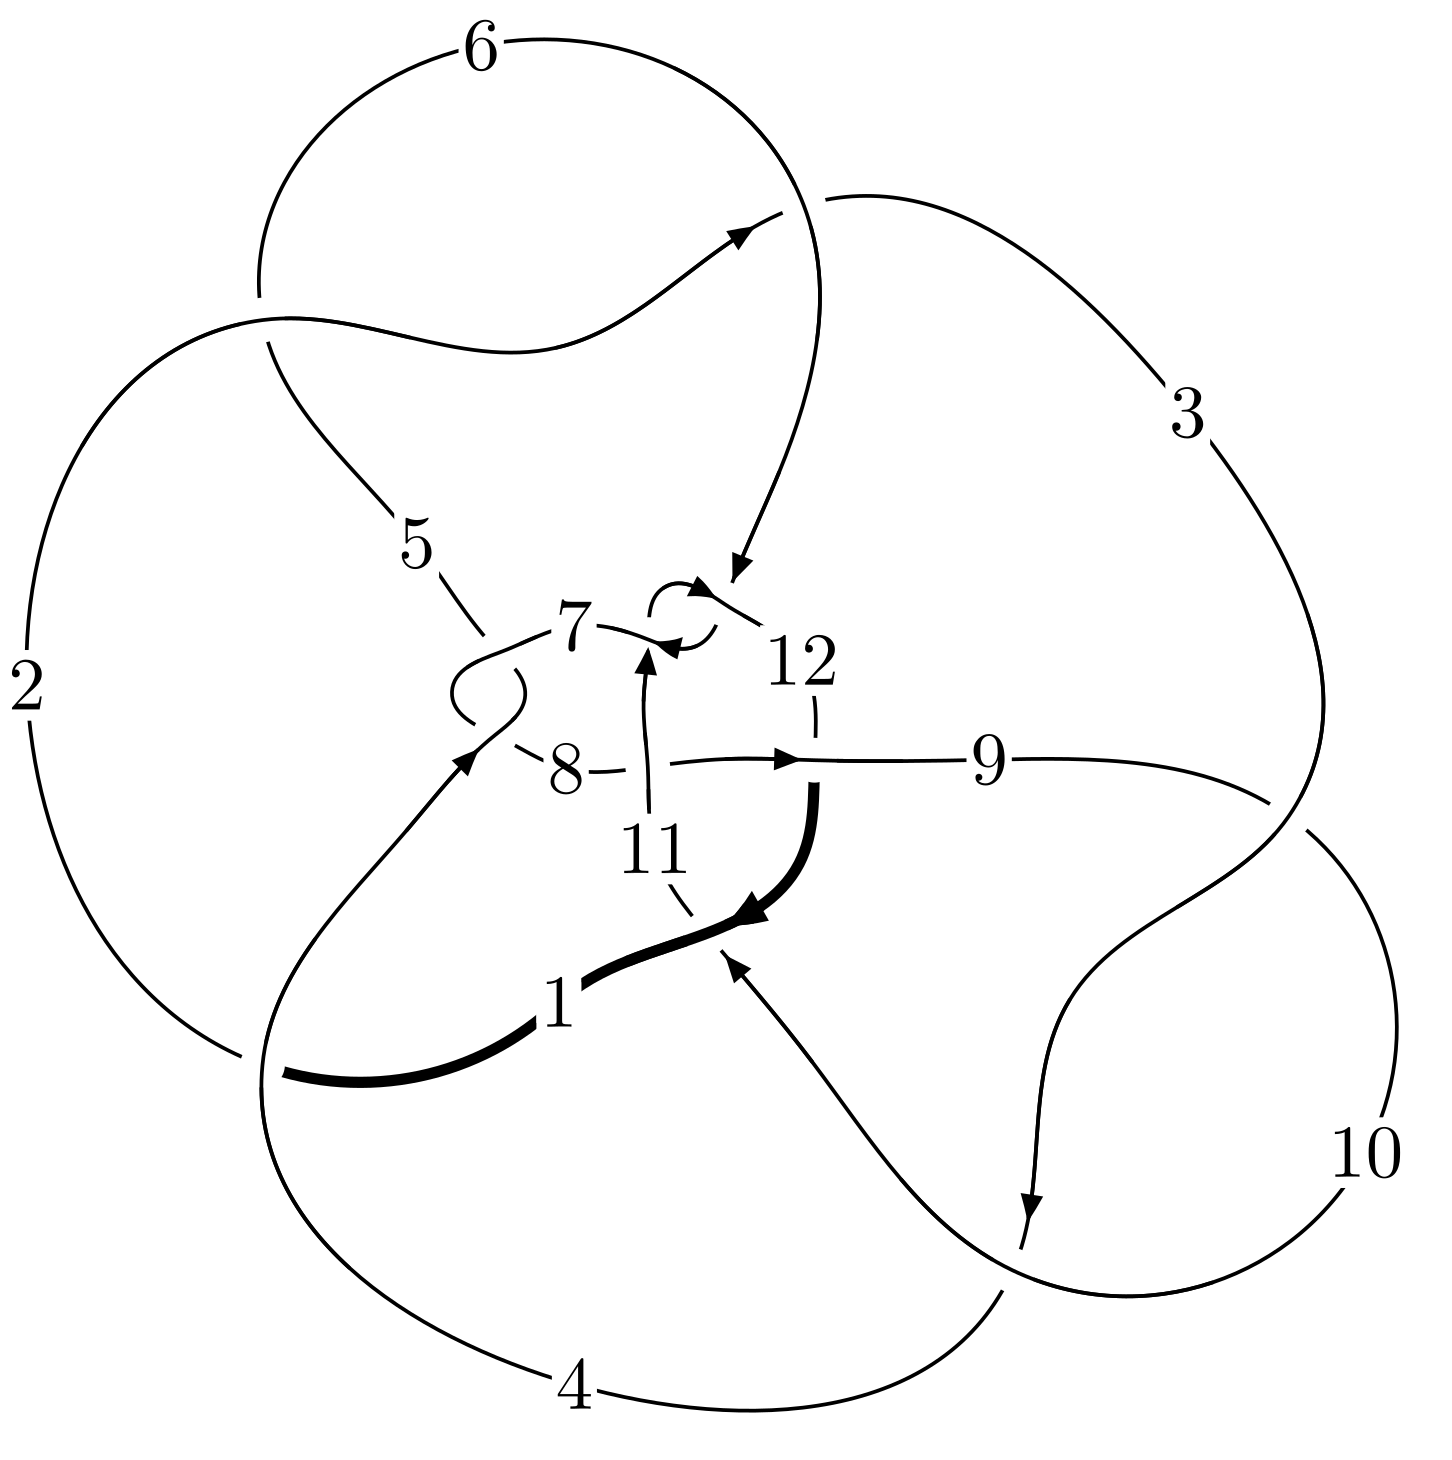
\includegraphics[width=112pt]{../../../GIT/diagram.site/Diagrams/png/2879_12n_0790.png}\\
\ \ \ A knot diagram\footnotemark}&
\allowdisplaybreaks
\textbf{Linearized knot diagam} \\
\cline{2-2}
 &
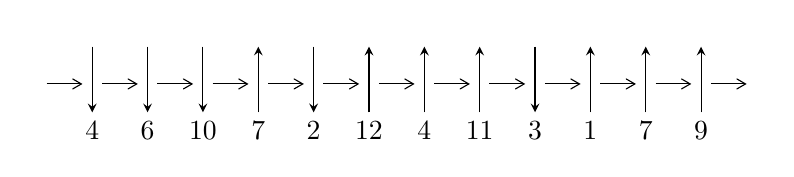
\begin{tikzpicture}[x=20pt, y=17pt]
	% nodes
	\node (C0) at (0, 0) {};
	\node (C1) at (1, 0) {};
	\node (C1U) at (1, +1) {};
	\node (C1D) at (1, -1) {4};

	\node (C2) at (2, 0) {};
	\node (C2U) at (2, +1) {};
	\node (C2D) at (2, -1) {6};

	\node (C3) at (3, 0) {};
	\node (C3U) at (3, +1) {};
	\node (C3D) at (3, -1) {10};

	\node (C4) at (4, 0) {};
	\node (C4U) at (4, +1) {};
	\node (C4D) at (4, -1) {7};

	\node (C5) at (5, 0) {};
	\node (C5U) at (5, +1) {};
	\node (C5D) at (5, -1) {2};

	\node (C6) at (6, 0) {};
	\node (C6U) at (6, +1) {};
	\node (C6D) at (6, -1) {12};

	\node (C7) at (7, 0) {};
	\node (C7U) at (7, +1) {};
	\node (C7D) at (7, -1) {4};

	\node (C8) at (8, 0) {};
	\node (C8U) at (8, +1) {};
	\node (C8D) at (8, -1) {11};

	\node (C9) at (9, 0) {};
	\node (C9U) at (9, +1) {};
	\node (C9D) at (9, -1) {3};

	\node (C10) at (10, 0) {};
	\node (C10U) at (10, +1) {};
	\node (C10D) at (10, -1) {1};

	\node (C11) at (11, 0) {};
	\node (C11U) at (11, +1) {};
	\node (C11D) at (11, -1) {7};

	\node (C12) at (12, 0) {};
	\node (C12U) at (12, +1) {};
	\node (C12D) at (12, -1) {9};
	\node (C13) at (13, 0) {};

	% arrows
	\draw[->,>={angle 60}]
	(C0) edge (C1) (C1) edge (C2) (C2) edge (C3) (C3) edge (C4) (C4) edge (C5) (C5) edge (C6) (C6) edge (C7) (C7) edge (C8) (C8) edge (C9) (C9) edge (C10) (C10) edge (C11) (C11) edge (C12) (C12) edge (C13) ;	\draw[->,>=stealth]
	(C1U) edge (C1D) (C2U) edge (C2D) (C3U) edge (C3D) (C4D) edge (C4U) (C5U) edge (C5D) (C6D) edge (C6U) (C7D) edge (C7U) (C8D) edge (C8U) (C9U) edge (C9D) (C10D) edge (C10U) (C11D) edge (C11U) (C12D) edge (C12U) ;
	\end{tikzpicture} \\
\hhline{~~} \\& 
\textbf{Solving Sequence} \\ \cline{2-2} 
 &
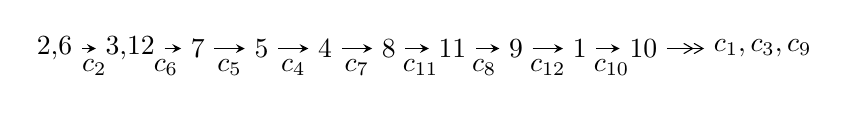
\begin{tikzpicture}[x=23pt, y=7pt]
	% node
	\node (A0) at (-1/8, 0) {2,6};
	\node (A1) at (17/16, 0) {3,12};
	\node (A2) at (17/8, 0) {7};
	\node (A3) at (25/8, 0) {5};
	\node (A4) at (33/8, 0) {4};
	\node (A5) at (41/8, 0) {8};
	\node (A6) at (49/8, 0) {11};
	\node (A7) at (57/8, 0) {9};
	\node (A8) at (65/8, 0) {1};
	\node (A9) at (73/8, 0) {10};
	\node (C1) at (1/2, -1) {$c_{2}$};
	\node (C2) at (13/8, -1) {$c_{6}$};
	\node (C3) at (21/8, -1) {$c_{5}$};
	\node (C4) at (29/8, -1) {$c_{4}$};
	\node (C5) at (37/8, -1) {$c_{7}$};
	\node (C6) at (45/8, -1) {$c_{11}$};
	\node (C7) at (53/8, -1) {$c_{8}$};
	\node (C8) at (61/8, -1) {$c_{12}$};
	\node (C9) at (69/8, -1) {$c_{10}$};
	\node (A10) at (11, 0) {$c_{1},c_{3},c_{9}$};

	% edge
	\draw[->,>=stealth]	
	(A0) edge (A1) (A1) edge (A2) (A2) edge (A3) (A3) edge (A4) (A4) edge (A5) (A5) edge (A6) (A6) edge (A7) (A7) edge (A8) (A8) edge (A9) ;
	\draw[->>,>={angle 60}]	
	(A9) edge (A10);
\end{tikzpicture} \\ 

\end{tabular} \\

\footnotetext{
The image of knot diagram is generated by the software ``\textbf{Draw programme}" developed by Andrew Bartholomew(\url{http://www.layer8.co.uk/maths/draw/index.htm\#Running-draw}), where we modified some parts for our purpose(\url{https://github.com/CATsTAILs/LinksPainter}).
}\phantom \\ \newline 
\centering \textbf{Ideals for irreducible components\footnotemark of $X_{\text{par}}$} 
 
\begin{align*}
I^u_{1}&=\langle 
-7.14667\times10^{409} u^{92}-5.32523\times10^{410} u^{91}+\cdots+4.98001\times10^{410} b-3.89130\times10^{412},\\
\phantom{I^u_{1}}&\phantom{= \langle  }4.70081\times10^{411} u^{92}+3.48169\times10^{412} u^{91}+\cdots+3.46111\times10^{413} a+1.89968\times10^{415},\\
\phantom{I^u_{1}}&\phantom{= \langle  }3 u^{93}+22 u^{92}+\cdots+6023 u+695\rangle \\
I^u_{2}&=\langle 
-5.47528\times10^{24} u^{26}-9.23714\times10^{22} u^{25}+\cdots+2.62202\times10^{24} b-3.76400\times10^{22},\\
\phantom{I^u_{2}}&\phantom{= \langle  }-2.17634\times10^{24} u^{26}+3.10319\times10^{24} u^{25}+\cdots+2.62202\times10^{24} a-1.13279\times10^{25},\;3 u^{27}- u^{26}+\cdots-6 u^2+1\rangle \\
\\
\end{align*}
\raggedright * 2 irreducible components of $\dim_{\mathbb{C}}=0$, with total 120 representations.\\
\footnotetext{All coefficients of polynomials are rational numbers. But the coefficients are sometimes approximated in decimal forms when there is not enough margin.}
\newpage
\renewcommand{\arraystretch}{1}
\centering \section*{I. $I^u_{1}= \langle -7.15\times10^{409} u^{92}-5.33\times10^{410} u^{91}+\cdots+4.98\times10^{410} b-3.89\times10^{412},\;4.70\times10^{411} u^{92}+3.48\times10^{412} u^{91}+\cdots+3.46\times10^{413} a+1.90\times10^{415},\;3 u^{93}+22 u^{92}+\cdots+6023 u+695 \rangle$}
\flushleft \textbf{(i) Arc colorings}\\
\begin{tabular}{m{7pt} m{180pt} m{7pt} m{180pt} }
\flushright $a_{2}=$&$\begin{pmatrix}1\\0\end{pmatrix}$ \\
\flushright $a_{6}=$&$\begin{pmatrix}0\\u\end{pmatrix}$ \\
\flushright $a_{3}=$&$\begin{pmatrix}1\\u^2\end{pmatrix}$ \\
\flushright $a_{12}=$&$\begin{pmatrix}-0.0135818 u^{92}-0.100595 u^{91}+\cdots-238.687 u-54.8864\\0.143507 u^{92}+1.06932 u^{91}+\cdots+568.056 u+78.1384\end{pmatrix}$ \\
\flushright $a_{7}=$&$\begin{pmatrix}-0.301700 u^{92}-2.00007 u^{91}+\cdots-550.015 u-80.7225\\-0.295411 u^{92}-1.99275 u^{91}+\cdots-598.971 u-73.2675\end{pmatrix}$ \\
\flushright $a_{5}=$&$\begin{pmatrix}u\\u\end{pmatrix}$ \\
\flushright $a_{4}=$&$\begin{pmatrix}0.0629549 u^{92}+0.517586 u^{91}+\cdots+447.875 u+108.119\\-0.0833166 u^{92}-0.479335 u^{91}+\cdots+1.31628 u+2.37199\end{pmatrix}$ \\
\flushright $a_{8}=$&$\begin{pmatrix}-0.185984 u^{92}-1.41044 u^{91}+\cdots-1066.72 u-289.305\\-0.0386972 u^{92}-0.308193 u^{91}+\cdots-77.2777 u-1.02321\end{pmatrix}$ \\
\flushright $a_{11}=$&$\begin{pmatrix}-0.382257 u^{92}-2.77588 u^{91}+\cdots-1845.24 u-324.691\\0.143790 u^{92}+0.957852 u^{91}+\cdots+265.817 u+30.9818\end{pmatrix}$ \\
\flushright $a_{9}=$&$\begin{pmatrix}0.127751 u^{92}+0.819530 u^{91}+\cdots+175.460 u-2.90117\\0.152700 u^{92}+1.01579 u^{91}+\cdots+335.904 u+44.8910\end{pmatrix}$ \\
\flushright $a_{1}=$&$\begin{pmatrix}1.32557 u^{92}+8.92984 u^{91}+\cdots+3658.56 u+546.752\\0.468972 u^{92}+3.23240 u^{91}+\cdots+1446.79 u+205.465\end{pmatrix}$ \\
\flushright $a_{10}=$&$\begin{pmatrix}0.0625451 u^{92}+0.381060 u^{91}+\cdots+45.4867 u-20.6145\\0.141552 u^{92}+0.924644 u^{91}+\cdots+271.287 u+35.6916\end{pmatrix}$\\&\end{tabular}
\flushleft \textbf{(ii) Obstruction class $= -1$}\\~\\
\flushleft \textbf{(iii) Cusp Shapes $= 0.215998 u^{92}+1.15544 u^{91}+\cdots+644.040 u+222.694$}\\~\\
\newpage\renewcommand{\arraystretch}{1}
\flushleft \textbf{(iv) u-Polynomials at the component}\newline \\
\begin{tabular}{m{50pt}|m{274pt}}
Crossings & \hspace{64pt}u-Polynomials at each crossing \\
\hline $$\begin{aligned}c_{1}\end{aligned}$$&$\begin{aligned}
&u^{93}+u^{92}+\cdots-493754 u-46509
\end{aligned}$\\
\hline $$\begin{aligned}c_{2},c_{5}\end{aligned}$$&$\begin{aligned}
&3(3 u^{93}+22 u^{92}+\cdots+6023 u+695)
\end{aligned}$\\
\hline $$\begin{aligned}c_{3},c_{9}\end{aligned}$$&$\begin{aligned}
&u^{93}-4 u^{92}+\cdots-435 u+281
\end{aligned}$\\
\hline $$\begin{aligned}c_{4},c_{7}\end{aligned}$$&$\begin{aligned}
&u^{93}+9 u^{92}+\cdots-341511 u-15167
\end{aligned}$\\
\hline $$\begin{aligned}c_{6},c_{11}\end{aligned}$$&$\begin{aligned}
&3(3 u^{93}-5 u^{92}+\cdots-24386 u-2531)
\end{aligned}$\\
\hline $$\begin{aligned}c_{8}\end{aligned}$$&$\begin{aligned}
&u^{93}+16 u^{92}+\cdots+256813 u+72465
\end{aligned}$\\
\hline $$\begin{aligned}c_{10}\end{aligned}$$&$\begin{aligned}
&9(9 u^{93}+71 u^{92}+\cdots-6 u-1)
\end{aligned}$\\
\hline $$\begin{aligned}c_{12}\end{aligned}$$&$\begin{aligned}
&u^{93}+3 u^{91}+\cdots+17755 u+2097
\end{aligned}$\\
\hline
\end{tabular}\\~\\
\newpage\renewcommand{\arraystretch}{1}
\flushleft \textbf{(v) Riley Polynomials at the component}\newline \\
\begin{tabular}{m{50pt}|m{274pt}}
Crossings & \hspace{64pt}Riley Polynomials at each crossing \\
\hline $$\begin{aligned}c_{1}\end{aligned}$$&$\begin{aligned}
&y^{93}+7 y^{92}+\cdots-70016139986 y-2163087081
\end{aligned}$\\
\hline $$\begin{aligned}c_{2},c_{5}\end{aligned}$$&$\begin{aligned}
&9(9 y^{93}-298 y^{92}+\cdots+1.07075\times10^{7} y-483025)
\end{aligned}$\\
\hline $$\begin{aligned}c_{3},c_{9}\end{aligned}$$&$\begin{aligned}
&y^{93}-62 y^{92}+\cdots+1260959 y-78961
\end{aligned}$\\
\hline $$\begin{aligned}c_{4},c_{7}\end{aligned}$$&$\begin{aligned}
&y^{93}-81 y^{92}+\cdots-1602188993 y-230037889
\end{aligned}$\\
\hline $$\begin{aligned}c_{6},c_{11}\end{aligned}$$&$\begin{aligned}
&9(9 y^{93}+395 y^{92}+\cdots-7.45852\times10^{7} y-6405961)
\end{aligned}$\\
\hline $$\begin{aligned}c_{8}\end{aligned}$$&$\begin{aligned}
&y^{93}-42 y^{92}+\cdots+228494230849 y-5251176225
\end{aligned}$\\
\hline $$\begin{aligned}c_{10}\end{aligned}$$&$\begin{aligned}
&81(81 y^{93}-1621 y^{92}+\cdots-20 y-1)
\end{aligned}$\\
\hline $$\begin{aligned}c_{12}\end{aligned}$$&$\begin{aligned}
&y^{93}+6 y^{92}+\cdots+66493885 y-4397409
\end{aligned}$\\
\hline
\end{tabular}\\~\\
\newpage\flushleft \textbf{(vi) Complex Volumes and Cusp Shapes}
$$\begin{array}{c|c|c}  
\text{Solutions to }I^u_{1}& \I (\text{vol} + \sqrt{-1}CS) & \text{Cusp shape}\\
 \hline 
\begin{aligned}
u &= \phantom{-}0.674954 + 0.732172 I \\
a &= \phantom{-}1.215980 - 0.268347 I \\
b &= \phantom{-}0.139557 + 0.583522 I\end{aligned}
 & \phantom{-}2.81000 + 0.59876 I & \phantom{-0.000000 } 0 \\ \hline\begin{aligned}
u &= \phantom{-}0.674954 - 0.732172 I \\
a &= \phantom{-}1.215980 + 0.268347 I \\
b &= \phantom{-}0.139557 - 0.583522 I\end{aligned}
 & \phantom{-}2.81000 - 0.59876 I & \phantom{-0.000000 } 0 \\ \hline\begin{aligned}
u &= \phantom{-}0.686494 + 0.697906 I \\
a &= -0.001348 - 1.067160 I \\
b &= \phantom{-}1.10088 - 2.50838 I\end{aligned}
 & \phantom{-}2.54150 - 7.26629 I & \phantom{-0.000000 } 0 \\ \hline\begin{aligned}
u &= \phantom{-}0.686494 - 0.697906 I \\
a &= -0.001348 + 1.067160 I \\
b &= \phantom{-}1.10088 + 2.50838 I\end{aligned}
 & \phantom{-}2.54150 + 7.26629 I & \phantom{-0.000000 } 0 \\ \hline\begin{aligned}
u &= -0.691333 + 0.690971 I \\
a &= \phantom{-}0.346050 - 1.118080 I \\
b &= \phantom{-}0.103808 - 0.667560 I\end{aligned}
 & -1.23938 + 3.77370 I & \phantom{-0.000000 } 0 \\ \hline\begin{aligned}
u &= -0.691333 - 0.690971 I \\
a &= \phantom{-}0.346050 + 1.118080 I \\
b &= \phantom{-}0.103808 + 0.667560 I\end{aligned}
 & -1.23938 - 3.77370 I & \phantom{-0.000000 } 0 \\ \hline\begin{aligned}
u &= -0.937905 + 0.192409 I \\
a &= \phantom{-}0.198382 + 0.296203 I \\
b &= -0.638617 + 0.629199 I\end{aligned}
 & -1.61133 + 0.24005 I & \phantom{-0.000000 } 0 \\ \hline\begin{aligned}
u &= -0.937905 - 0.192409 I \\
a &= \phantom{-}0.198382 - 0.296203 I \\
b &= -0.638617 - 0.629199 I\end{aligned}
 & -1.61133 - 0.24005 I & \phantom{-0.000000 } 0 \\ \hline\begin{aligned}
u &= -0.948386 + 0.462059 I \\
a &= -0.133432 + 0.734649 I \\
b &= -0.660912 + 0.952450 I\end{aligned}
 & -2.50321 + 0.81346 I & \phantom{-0.000000 } 0 \\ \hline\begin{aligned}
u &= -0.948386 - 0.462059 I \\
a &= -0.133432 - 0.734649 I \\
b &= -0.660912 - 0.952450 I\end{aligned}
 & -2.50321 - 0.81346 I & \phantom{-0.000000 } 0\\
 \hline 
 \end{array}$$\newpage$$\begin{array}{c|c|c}  
\text{Solutions to }I^u_{1}& \I (\text{vol} + \sqrt{-1}CS) & \text{Cusp shape}\\
 \hline 
\begin{aligned}
u &= \phantom{-}0.095269 + 0.938474 I \\
a &= \phantom{-}0.473851 + 0.415001 I \\
b &= \phantom{-}0.512383 - 0.773209 I\end{aligned}
 & \phantom{-}2.00771 - 3.44099 I & \phantom{-0.000000 } 0 \\ \hline\begin{aligned}
u &= \phantom{-}0.095269 - 0.938474 I \\
a &= \phantom{-}0.473851 - 0.415001 I \\
b &= \phantom{-}0.512383 + 0.773209 I\end{aligned}
 & \phantom{-}2.00771 + 3.44099 I & \phantom{-0.000000 } 0 \\ \hline\begin{aligned}
u &= \phantom{-}0.823460 + 0.375542 I \\
a &= -0.119724 - 1.144210 I \\
b &= -1.03275 - 1.35723 I\end{aligned}
 & -6.20249 - 5.22443 I & \phantom{-0.000000 } 0 \\ \hline\begin{aligned}
u &= \phantom{-}0.823460 - 0.375542 I \\
a &= -0.119724 + 1.144210 I \\
b &= -1.03275 + 1.35723 I\end{aligned}
 & -6.20249 + 5.22443 I & \phantom{-0.000000 } 0 \\ \hline\begin{aligned}
u &= \phantom{-}0.854498 + 0.689956 I \\
a &= \phantom{-}0.093394 + 0.958920 I \\
b &= -1.15625 + 1.81104 I\end{aligned}
 & \phantom{-}4.75042 - 0.26422 I & \phantom{-0.000000 } 0 \\ \hline\begin{aligned}
u &= \phantom{-}0.854498 - 0.689956 I \\
a &= \phantom{-}0.093394 - 0.958920 I \\
b &= -1.15625 - 1.81104 I\end{aligned}
 & \phantom{-}4.75042 + 0.26422 I & \phantom{-0.000000 } 0 \\ \hline\begin{aligned}
u &= \phantom{-}0.918476 + 0.606358 I \\
a &= -0.434023 - 0.634737 I \\
b &= -0.903200 - 0.654198 I\end{aligned}
 & -5.81791 + 4.00342 I & \phantom{-0.000000 } 0 \\ \hline\begin{aligned}
u &= \phantom{-}0.918476 - 0.606358 I \\
a &= -0.434023 + 0.634737 I \\
b &= -0.903200 + 0.654198 I\end{aligned}
 & -5.81791 - 4.00342 I & \phantom{-0.000000 } 0 \\ \hline\begin{aligned}
u &= \phantom{-}0.872877 + 0.109712 I \\
a &= -0.52784 + 1.37760 I \\
b &= \phantom{-}0.564876 + 0.849824 I\end{aligned}
 & -6.64115 + 3.23471 I & -7.67162 + 0. I\phantom{ +0.000000I} \\ \hline\begin{aligned}
u &= \phantom{-}0.872877 - 0.109712 I \\
a &= -0.52784 - 1.37760 I \\
b &= \phantom{-}0.564876 - 0.849824 I\end{aligned}
 & -6.64115 - 3.23471 I & -7.67162 + 0. I\phantom{ +0.000000I}\\
 \hline 
 \end{array}$$\newpage$$\begin{array}{c|c|c}  
\text{Solutions to }I^u_{1}& \I (\text{vol} + \sqrt{-1}CS) & \text{Cusp shape}\\
 \hline 
\begin{aligned}
u &= \phantom{-}0.878160 + 0.700675 I \\
a &= -1.086750 + 0.245560 I \\
b &= -0.028345 - 0.641744 I\end{aligned}
 & \phantom{-}4.67143 - 5.07155 I & \phantom{-0.000000 } 0 \\ \hline\begin{aligned}
u &= \phantom{-}0.878160 - 0.700675 I \\
a &= -1.086750 - 0.245560 I \\
b &= -0.028345 + 0.641744 I\end{aligned}
 & \phantom{-}4.67143 + 5.07155 I & \phantom{-0.000000 } 0 \\ \hline\begin{aligned}
u &= -0.662848 + 0.569436 I \\
a &= -0.071156 - 0.971664 I \\
b &= -1.63900 - 1.99223 I\end{aligned}
 & \phantom{-}2.25029 - 5.38425 I & \phantom{-0.000000 } 0 \\ \hline\begin{aligned}
u &= -0.662848 - 0.569436 I \\
a &= -0.071156 + 0.971664 I \\
b &= -1.63900 + 1.99223 I\end{aligned}
 & \phantom{-}2.25029 + 5.38425 I & \phantom{-0.000000 } 0 \\ \hline\begin{aligned}
u &= -1.128720 + 0.149564 I \\
a &= \phantom{-}0.30651 - 1.52316 I \\
b &= \phantom{-}0.02115 - 1.67361 I\end{aligned}
 & -8.96468 - 3.92565 I & \phantom{-0.000000 } 0 \\ \hline\begin{aligned}
u &= -1.128720 - 0.149564 I \\
a &= \phantom{-}0.30651 + 1.52316 I \\
b &= \phantom{-}0.02115 + 1.67361 I\end{aligned}
 & -8.96468 + 3.92565 I & \phantom{-0.000000 } 0 \\ \hline\begin{aligned}
u &= \phantom{-}0.398460 + 0.758184 I \\
a &= \phantom{-}1.077610 - 0.881690 I \\
b &= \phantom{-}0.344671 + 0.364720 I\end{aligned}
 & \phantom{-}3.37801 + 0.99096 I & \phantom{-}6.48497 + 0. I\phantom{ +0.000000I} \\ \hline\begin{aligned}
u &= \phantom{-}0.398460 - 0.758184 I \\
a &= \phantom{-}1.077610 + 0.881690 I \\
b &= \phantom{-}0.344671 - 0.364720 I\end{aligned}
 & \phantom{-}3.37801 - 0.99096 I & \phantom{-}6.48497 + 0. I\phantom{ +0.000000I} \\ \hline\begin{aligned}
u &= \phantom{-}0.933778 + 0.704004 I \\
a &= -0.091450 + 1.054630 I \\
b &= -0.010874 + 0.746479 I\end{aligned}
 & -5.82082 - 9.31118 I & \phantom{-0.000000 } 0 \\ \hline\begin{aligned}
u &= \phantom{-}0.933778 - 0.704004 I \\
a &= -0.091450 - 1.054630 I \\
b &= -0.010874 - 0.746479 I\end{aligned}
 & -5.82082 + 9.31118 I & \phantom{-0.000000 } 0\\
 \hline 
 \end{array}$$\newpage$$\begin{array}{c|c|c}  
\text{Solutions to }I^u_{1}& \I (\text{vol} + \sqrt{-1}CS) & \text{Cusp shape}\\
 \hline 
\begin{aligned}
u &= -0.442517 + 0.688839 I \\
a &= \phantom{-}0.176317 + 0.822306 I \\
b &= \phantom{-}0.249277 + 0.829583 I\end{aligned}
 & -0.81738 + 3.68689 I & \phantom{-0.000000 } 0. - 7.64746 I \\ \hline\begin{aligned}
u &= -0.442517 - 0.688839 I \\
a &= \phantom{-}0.176317 - 0.822306 I \\
b &= \phantom{-}0.249277 - 0.829583 I\end{aligned}
 & -0.81738 - 3.68689 I & \phantom{-0.000000 -}0. + 7.64746 I \\ \hline\begin{aligned}
u &= -0.619214 + 0.521758 I \\
a &= \phantom{-}0.742330 + 0.106731 I \\
b &= -0.113697 + 0.262021 I\end{aligned}
 & -1.67952 + 0.53410 I & -4.21973 + 0. I\phantom{ +0.000000I} \\ \hline\begin{aligned}
u &= -0.619214 - 0.521758 I \\
a &= \phantom{-}0.742330 - 0.106731 I \\
b &= -0.113697 - 0.262021 I\end{aligned}
 & -1.67952 - 0.53410 I & -4.21973 + 0. I\phantom{ +0.000000I} \\ \hline\begin{aligned}
u &= \phantom{-}1.112030 + 0.426697 I \\
a &= \phantom{-}0.084200 - 1.167710 I \\
b &= -0.10451 - 1.58436 I\end{aligned}
 & -5.26330 - 4.96135 I & \phantom{-0.000000 } 0 \\ \hline\begin{aligned}
u &= \phantom{-}1.112030 - 0.426697 I \\
a &= \phantom{-}0.084200 + 1.167710 I \\
b &= -0.10451 + 1.58436 I\end{aligned}
 & -5.26330 + 4.96135 I & \phantom{-0.000000 } 0 \\ \hline\begin{aligned}
u &= -0.623299 + 0.503573 I \\
a &= -0.92680 + 1.62860 I \\
b &= -0.40002 + 2.17351 I\end{aligned}
 & -6.65496 + 6.93046 I & \phantom{-0.000000 } 0. - 11.05037 I \\ \hline\begin{aligned}
u &= -0.623299 - 0.503573 I \\
a &= -0.92680 - 1.62860 I \\
b &= -0.40002 - 2.17351 I\end{aligned}
 & -6.65496 - 6.93046 I & \phantom{-0.000000 -}0. + 11.05037 I \\ \hline\begin{aligned}
u &= -0.692093 + 0.397215 I \\
a &= -0.099142 + 0.920873 I \\
b &= \phantom{-}1.81566 + 1.93139 I\end{aligned}
 & \phantom{-}2.87496 + 2.75738 I & -1.61500 - 5.30010 I \\ \hline\begin{aligned}
u &= -0.692093 - 0.397215 I \\
a &= -0.099142 - 0.920873 I \\
b &= \phantom{-}1.81566 - 1.93139 I\end{aligned}
 & \phantom{-}2.87496 - 2.75738 I & -1.61500 + 5.30010 I\\
 \hline 
 \end{array}$$\newpage$$\begin{array}{c|c|c}  
\text{Solutions to }I^u_{1}& \I (\text{vol} + \sqrt{-1}CS) & \text{Cusp shape}\\
 \hline 
\begin{aligned}
u &= -1.044320 + 0.596872 I \\
a &= -1.300970 - 0.184765 I \\
b &= -0.170854 + 0.517420 I\end{aligned}
 & \phantom{-}0.96308 + 10.07780 I & \phantom{-0.000000 } 0 \\ \hline\begin{aligned}
u &= -1.044320 - 0.596872 I \\
a &= -1.300970 + 0.184765 I \\
b &= -0.170854 - 0.517420 I\end{aligned}
 & \phantom{-}0.96308 - 10.07780 I & \phantom{-0.000000 } 0 \\ \hline\begin{aligned}
u &= -1.083630 + 0.537499 I \\
a &= -0.070934 + 1.305290 I \\
b &= \phantom{-}0.85778 + 1.95035 I\end{aligned}
 & -0.80241 + 7.59723 I & \phantom{-0.000000 } 0 \\ \hline\begin{aligned}
u &= -1.083630 - 0.537499 I \\
a &= -0.070934 - 1.305290 I \\
b &= \phantom{-}0.85778 - 1.95035 I\end{aligned}
 & -0.80241 - 7.59723 I & \phantom{-0.000000 } 0 \\ \hline\begin{aligned}
u &= \phantom{-}0.733455 + 0.252583 I \\
a &= -0.30543 - 1.82531 I \\
b &= \phantom{-}0.00457 - 2.01689 I\end{aligned}
 & -4.01462 - 3.43234 I & \phantom{-}8.55484 + 7.50603 I \\ \hline\begin{aligned}
u &= \phantom{-}0.733455 - 0.252583 I \\
a &= -0.30543 + 1.82531 I \\
b &= \phantom{-}0.00457 + 2.01689 I\end{aligned}
 & -4.01462 + 3.43234 I & \phantom{-}8.55484 - 7.50603 I \\ \hline\begin{aligned}
u &= -1.24771\phantom{ +0.000000I} \\
a &= \phantom{-}0.914123\phantom{ +0.000000I} \\
b &= -0.758760\phantom{ +0.000000I}\end{aligned}
 & \phantom{-}0.556605\phantom{ +0.000000I} & \phantom{-0.000000 } 0 \\ \hline\begin{aligned}
u &= \phantom{-}1.089900 + 0.607822 I \\
a &= \phantom{-}0.181194 - 1.176140 I \\
b &= \phantom{-}0.94657 - 1.94638 I\end{aligned}
 & \phantom{-}1.36282 - 6.16551 I & \phantom{-0.000000 } 0 \\ \hline\begin{aligned}
u &= \phantom{-}1.089900 - 0.607822 I \\
a &= \phantom{-}0.181194 + 1.176140 I \\
b &= \phantom{-}0.94657 + 1.94638 I\end{aligned}
 & \phantom{-}1.36282 + 6.16551 I & \phantom{-0.000000 } 0 \\ \hline\begin{aligned}
u &= \phantom{-}1.264290 + 0.183174 I \\
a &= \phantom{-}0.479294 - 0.545939 I \\
b &= -0.381207 - 0.859789 I\end{aligned}
 & -2.91671 - 0.62225 I & \phantom{-0.000000 } 0\\
 \hline 
 \end{array}$$\newpage$$\begin{array}{c|c|c}  
\text{Solutions to }I^u_{1}& \I (\text{vol} + \sqrt{-1}CS) & \text{Cusp shape}\\
 \hline 
\begin{aligned}
u &= \phantom{-}1.264290 - 0.183174 I \\
a &= \phantom{-}0.479294 + 0.545939 I \\
b &= -0.381207 + 0.859789 I\end{aligned}
 & -2.91671 + 0.62225 I & \phantom{-0.000000 } 0 \\ \hline\begin{aligned}
u &= -0.910304 + 0.900507 I \\
a &= \phantom{-}0.522542 - 1.020090 I \\
b &= -0.74377 - 1.38645 I\end{aligned}
 & -2.57873 + 6.21327 I & \phantom{-0.000000 } 0 \\ \hline\begin{aligned}
u &= -0.910304 - 0.900507 I \\
a &= \phantom{-}0.522542 + 1.020090 I \\
b &= -0.74377 + 1.38645 I\end{aligned}
 & -2.57873 - 6.21327 I & \phantom{-0.000000 } 0 \\ \hline\begin{aligned}
u &= \phantom{-}1.119580 + 0.704429 I \\
a &= \phantom{-}0.089214 - 1.066460 I \\
b &= \phantom{-}0.79897 - 1.96272 I\end{aligned}
 & \phantom{-}1.49803 - 6.24365 I & \phantom{-0.000000 } 0 \\ \hline\begin{aligned}
u &= \phantom{-}1.119580 - 0.704429 I \\
a &= \phantom{-}0.089214 + 1.066460 I \\
b &= \phantom{-}0.79897 + 1.96272 I\end{aligned}
 & \phantom{-}1.49803 + 6.24365 I & \phantom{-0.000000 } 0 \\ \hline\begin{aligned}
u &= -0.588087 + 0.331536 I \\
a &= \phantom{-}1.83719 - 0.13136 I \\
b &= \phantom{-}0.125737 - 1.152850 I\end{aligned}
 & \phantom{-}1.12788 - 3.60271 I & \phantom{-}1.12062 + 5.92083 I \\ \hline\begin{aligned}
u &= -0.588087 - 0.331536 I \\
a &= \phantom{-}1.83719 + 0.13136 I \\
b &= \phantom{-}0.125737 + 1.152850 I\end{aligned}
 & \phantom{-}1.12788 + 3.60271 I & \phantom{-}1.12062 - 5.92083 I \\ \hline\begin{aligned}
u &= -1.203700 + 0.590086 I \\
a &= -0.347750 + 0.718485 I \\
b &= -0.25721 + 1.84323 I\end{aligned}
 & -3.96714 + 0.38677 I & \phantom{-0.000000 } 0 \\ \hline\begin{aligned}
u &= -1.203700 - 0.590086 I \\
a &= -0.347750 - 0.718485 I \\
b &= -0.25721 - 1.84323 I\end{aligned}
 & -3.96714 - 0.38677 I & \phantom{-0.000000 } 0 \\ \hline\begin{aligned}
u &= -0.287732 + 1.319090 I \\
a &= \phantom{-}0.193631 + 0.189893 I \\
b &= \phantom{-}0.192982 - 0.234031 I\end{aligned}
 & \phantom{-}4.31204 + 3.39765 I & \phantom{-0.000000 } 0\\
 \hline 
 \end{array}$$\newpage$$\begin{array}{c|c|c}  
\text{Solutions to }I^u_{1}& \I (\text{vol} + \sqrt{-1}CS) & \text{Cusp shape}\\
 \hline 
\begin{aligned}
u &= -0.287732 - 1.319090 I \\
a &= \phantom{-}0.193631 - 0.189893 I \\
b &= \phantom{-}0.192982 + 0.234031 I\end{aligned}
 & \phantom{-}4.31204 - 3.39765 I & \phantom{-0.000000 } 0 \\ \hline\begin{aligned}
u &= \phantom{-}0.544638 + 0.306845 I \\
a &= \phantom{-}0.92896 + 1.85109 I \\
b &= \phantom{-}0.519502 + 1.298470 I\end{aligned}
 & -2.86298 + 2.13949 I & \phantom{-}0.67058 - 5.49562 I \\ \hline\begin{aligned}
u &= \phantom{-}0.544638 - 0.306845 I \\
a &= \phantom{-}0.92896 - 1.85109 I \\
b &= \phantom{-}0.519502 - 1.298470 I\end{aligned}
 & -2.86298 - 2.13949 I & \phantom{-}0.67058 + 5.49562 I \\ \hline\begin{aligned}
u &= -0.489317 + 1.296330 I \\
a &= -0.474834 + 0.068876 I \\
b &= \phantom{-}0.355242 + 0.882752 I\end{aligned}
 & -0.52324 + 2.36440 I & \phantom{-0.000000 } 0 \\ \hline\begin{aligned}
u &= -0.489317 - 1.296330 I \\
a &= -0.474834 - 0.068876 I \\
b &= \phantom{-}0.355242 - 0.882752 I\end{aligned}
 & -0.52324 - 2.36440 I & \phantom{-0.000000 } 0 \\ \hline\begin{aligned}
u &= -1.297460 + 0.490834 I \\
a &= \phantom{-}0.242981 + 0.811654 I \\
b &= \phantom{-}0.74306 + 1.50520 I\end{aligned}
 & \phantom{-}0.31354 + 2.51804 I & \phantom{-0.000000 } 0 \\ \hline\begin{aligned}
u &= -1.297460 - 0.490834 I \\
a &= \phantom{-}0.242981 - 0.811654 I \\
b &= \phantom{-}0.74306 - 1.50520 I\end{aligned}
 & \phantom{-}0.31354 - 2.51804 I & \phantom{-0.000000 } 0 \\ \hline\begin{aligned}
u &= -0.566170\phantom{ +0.000000I} \\
a &= \phantom{-}3.10038\phantom{ +0.000000I} \\
b &= \phantom{-}0.553177\phantom{ +0.000000I}\end{aligned}
 & \phantom{-}4.63798\phantom{ +0.000000I} & -11.5780\phantom{ +0.000000I} \\ \hline\begin{aligned}
u &= \phantom{-}0.48605 + 1.35102 I \\
a &= -0.634856 + 0.184510 I \\
b &= \phantom{-}0.272403 - 0.519347 I\end{aligned}
 & \phantom{-}5.10190 + 4.33232 I & \phantom{-0.000000 } 0 \\ \hline\begin{aligned}
u &= \phantom{-}0.48605 - 1.35102 I \\
a &= -0.634856 - 0.184510 I \\
b &= \phantom{-}0.272403 + 0.519347 I\end{aligned}
 & \phantom{-}5.10190 - 4.33232 I & \phantom{-0.000000 } 0\\
 \hline 
 \end{array}$$\newpage$$\begin{array}{c|c|c}  
\text{Solutions to }I^u_{1}& \I (\text{vol} + \sqrt{-1}CS) & \text{Cusp shape}\\
 \hline 
\begin{aligned}
u &= -0.401346 + 0.289584 I \\
a &= -1.36249 - 1.64357 I \\
b &= \phantom{-}0.467604 + 0.316991 I\end{aligned}
 & \phantom{-}1.39489 + 1.09605 I & \phantom{-}4.43393 - 5.59913 I \\ \hline\begin{aligned}
u &= -0.401346 - 0.289584 I \\
a &= -1.36249 + 1.64357 I \\
b &= \phantom{-}0.467604 - 0.316991 I\end{aligned}
 & \phantom{-}1.39489 - 1.09605 I & \phantom{-}4.43393 + 5.59913 I \\ \hline\begin{aligned}
u &= -1.52411 + 0.05080 I \\
a &= -0.138758 - 0.528352 I \\
b &= -0.11425 - 2.03470 I\end{aligned}
 & -3.77465 + 0.88656 I & \phantom{-0.000000 } 0 \\ \hline\begin{aligned}
u &= -1.52411 - 0.05080 I \\
a &= -0.138758 + 0.528352 I \\
b &= -0.11425 + 2.03470 I\end{aligned}
 & -3.77465 - 0.88656 I & \phantom{-0.000000 } 0 \\ \hline\begin{aligned}
u &= \phantom{-}1.29646 + 0.81005 I \\
a &= \phantom{-}0.006482 + 0.935911 I \\
b &= -0.78276 + 2.01410 I\end{aligned}
 & \phantom{-}2.45748 - 11.81670 I & \phantom{-0.000000 } 0 \\ \hline\begin{aligned}
u &= \phantom{-}1.29646 - 0.81005 I \\
a &= \phantom{-}0.006482 - 0.935911 I \\
b &= -0.78276 - 2.01410 I\end{aligned}
 & \phantom{-}2.45748 + 11.81670 I & \phantom{-0.000000 } 0 \\ \hline\begin{aligned}
u &= -1.32096 + 0.78025 I \\
a &= \phantom{-}0.162237 - 0.827746 I \\
b &= -0.89132 - 1.79515 I\end{aligned}
 & -3.29057 + 5.02576 I & \phantom{-0.000000 } 0 \\ \hline\begin{aligned}
u &= -1.32096 - 0.78025 I \\
a &= \phantom{-}0.162237 + 0.827746 I \\
b &= -0.89132 + 1.79515 I\end{aligned}
 & -3.29057 - 5.02576 I & \phantom{-0.000000 } 0 \\ \hline\begin{aligned}
u &= -0.64910 + 1.41700 I \\
a &= -0.793221 - 0.052665 I \\
b &= \phantom{-}0.142883 + 0.621132 I\end{aligned}
 & \phantom{-}0.62586 - 10.14570 I & \phantom{-0.000000 } 0 \\ \hline\begin{aligned}
u &= -0.64910 - 1.41700 I \\
a &= -0.793221 + 0.052665 I \\
b &= \phantom{-}0.142883 - 0.621132 I\end{aligned}
 & \phantom{-}0.62586 + 10.14570 I & \phantom{-0.000000 } 0\\
 \hline 
 \end{array}$$\newpage$$\begin{array}{c|c|c}  
\text{Solutions to }I^u_{1}& \I (\text{vol} + \sqrt{-1}CS) & \text{Cusp shape}\\
 \hline 
\begin{aligned}
u &= \phantom{-}1.54061 + 0.31502 I \\
a &= -0.232279 + 0.505844 I \\
b &= \phantom{-}0.26775 + 2.05575 I\end{aligned}
 & -7.67390 - 7.52480 I & \phantom{-0.000000 } 0 \\ \hline\begin{aligned}
u &= \phantom{-}1.54061 - 0.31502 I \\
a &= -0.232279 - 0.505844 I \\
b &= \phantom{-}0.26775 - 2.05575 I\end{aligned}
 & -7.67390 + 7.52480 I & \phantom{-0.000000 } 0 \\ \hline\begin{aligned}
u &= -1.30908 + 0.87953 I \\
a &= \phantom{-}0.023926 - 1.014740 I \\
b &= -0.69764 - 2.04274 I\end{aligned}
 & -1.6681 + 18.1685 I & \phantom{-0.000000 } 0 \\ \hline\begin{aligned}
u &= -1.30908 - 0.87953 I \\
a &= \phantom{-}0.023926 + 1.014740 I \\
b &= -0.69764 + 2.04274 I\end{aligned}
 & -1.6681 - 18.1685 I & \phantom{-0.000000 } 0 \\ \hline\begin{aligned}
u &= -1.33446 + 0.96768 I \\
a &= -0.024479 + 0.973454 I \\
b &= \phantom{-}0.48958 + 1.98070 I\end{aligned}
 & -2.11305 + 8.95351 I & \phantom{-0.000000 } 0 \\ \hline\begin{aligned}
u &= -1.33446 - 0.96768 I \\
a &= -0.024479 - 0.973454 I \\
b &= \phantom{-}0.48958 - 1.98070 I\end{aligned}
 & -2.11305 - 8.95351 I & \phantom{-0.000000 } 0 \\ \hline\begin{aligned}
u &= -0.281062\phantom{ +0.000000I} \\
a &= -5.70017\phantom{ +0.000000I} \\
b &= \phantom{-}0.206328\phantom{ +0.000000I}\end{aligned}
 & \phantom{-}3.03653\phantom{ +0.000000I} & \phantom{-}44.5000\phantom{ +0.000000I} \\ \hline\begin{aligned}
u &= \phantom{-}0.107451 + 0.239477 I \\
a &= \phantom{-}0.35135 - 2.35992 I \\
b &= \phantom{-}0.433352 - 0.347109 I\end{aligned}
 & \phantom{-}1.228090 - 0.380559 I & \phantom{-}7.84885 + 1.47754 I \\ \hline\begin{aligned}
u &= \phantom{-}0.107451 - 0.239477 I \\
a &= \phantom{-}0.35135 + 2.35992 I \\
b &= \phantom{-}0.433352 + 0.347109 I\end{aligned}
 & \phantom{-}1.228090 + 0.380559 I & \phantom{-}7.84885 - 1.47754 I \\ \hline\begin{aligned}
u &= \phantom{-}1.75201 + 0.13606 I \\
a &= -0.132922 - 0.636322 I \\
b &= \phantom{-}0.11294 - 1.75128 I\end{aligned}
 & -9.64128 - 4.45809 I & \phantom{-0.000000 } 0\\
 \hline 
 \end{array}$$\newpage$$\begin{array}{c|c|c}  
\text{Solutions to }I^u_{1}& \I (\text{vol} + \sqrt{-1}CS) & \text{Cusp shape}\\
 \hline 
\begin{aligned}
u &= \phantom{-}1.75201 - 0.13606 I \\
a &= -0.132922 + 0.636322 I \\
b &= \phantom{-}0.11294 + 1.75128 I\end{aligned}
 & -9.64128 + 4.45809 I & \phantom{-0.000000 } 0 \\ \hline\begin{aligned}
u &= -0.61216 + 1.97687 I \\
a &= \phantom{-}0.972313 - 0.030847 I \\
b &= \phantom{-}0.143611 - 0.184027 I\end{aligned}
 & -0.0900114 - 0.0409964 I & \phantom{-0.000000 } 0 \\ \hline\begin{aligned}
u &= -0.61216 - 1.97687 I \\
a &= \phantom{-}0.972313 + 0.030847 I \\
b &= \phantom{-}0.143611 + 0.184027 I\end{aligned}
 & -0.0900114 + 0.0409964 I & \phantom{-0.000000 } 0\\
 \hline 
 \end{array}$$\newpage\newpage\renewcommand{\arraystretch}{1}
\centering \section*{II. $I^u_{2}= \langle -5.48\times10^{24} u^{26}-9.24\times10^{22} u^{25}+\cdots+2.62\times10^{24} b-3.76\times10^{22},\;-2.18\times10^{24} u^{26}+3.10\times10^{24} u^{25}+\cdots+2.62\times10^{24} a-1.13\times10^{25},\;3 u^{27}- u^{26}+\cdots-6 u^2+1 \rangle$}
\flushleft \textbf{(i) Arc colorings}\\
\begin{tabular}{m{7pt} m{180pt} m{7pt} m{180pt} }
\flushright $a_{2}=$&$\begin{pmatrix}1\\0\end{pmatrix}$ \\
\flushright $a_{6}=$&$\begin{pmatrix}0\\u\end{pmatrix}$ \\
\flushright $a_{3}=$&$\begin{pmatrix}1\\u^2\end{pmatrix}$ \\
\flushright $a_{12}=$&$\begin{pmatrix}0.830026 u^{26}-1.18351 u^{25}+\cdots-2.18146 u+4.32029\\2.08819 u^{26}+0.0352291 u^{25}+\cdots-0.969498 u+0.0143553\end{pmatrix}$ \\
\flushright $a_{7}=$&$\begin{pmatrix}-9.13895 u^{26}+3.75782 u^{25}+\cdots+19.1051 u-0.580350\\-1.21146 u^{26}+1.36298 u^{25}+\cdots+3.45375 u-0.913452\end{pmatrix}$ \\
\flushright $a_{5}=$&$\begin{pmatrix}u\\u\end{pmatrix}$ \\
\flushright $a_{4}=$&$\begin{pmatrix}19.8999 u^{26}-5.44200 u^{25}+\cdots-42.0029 u-0.818310\\2.13751 u^{26}-0.640341 u^{25}+\cdots-4.97331 u+0.983879\end{pmatrix}$ \\
\flushright $a_{8}=$&$\begin{pmatrix}-53.2973 u^{26}+14.6786 u^{25}+\cdots+116.922 u+3.66324\\-4.77966 u^{26}+2.89122 u^{25}+\cdots+13.8959 u-3.34107\end{pmatrix}$ \\
\flushright $a_{11}=$&$\begin{pmatrix}-0.703685 u^{26}-7.82470 u^{25}+\cdots-4.38591 u+16.7491\\1.55379 u^{26}-2.01157 u^{25}+\cdots-2.08747 u+1.79186\end{pmatrix}$ \\
\flushright $a_{9}=$&$\begin{pmatrix}-17.4160 u^{26}+6.20552 u^{25}+\cdots+38.6101 u-3.38199\\-2.41028 u^{26}+1.11206 u^{25}+\cdots+5.03666 u-0.825501\end{pmatrix}$ \\
\flushright $a_{1}=$&$\begin{pmatrix}-19.9953 u^{26}+17.9764 u^{25}+\cdots+47.8550 u-26.3512\\-4.73532 u^{26}+3.06498 u^{25}+\cdots+11.6086 u-4.04184\end{pmatrix}$ \\
\flushright $a_{10}=$&$\begin{pmatrix}-18.0474 u^{26}+6.17298 u^{25}+\cdots+39.3788 u-2.68988\\-2.60784 u^{26}+1.19707 u^{25}+\cdots+5.24713 u-0.744502\end{pmatrix}$\\&\end{tabular}
\flushleft \textbf{(ii) Obstruction class $= 1$}\\~\\
\flushleft \textbf{(iii) Cusp Shapes $= \frac{96546149137055527549848081}{2622017778319800888275503} u^{26}-\frac{21368440923253031371319385}{2622017778319800888275503} u^{25}+\cdots-\frac{206442519224589606723744388}{2622017778319800888275503} u-\frac{13602696470375884795425211}{2622017778319800888275503}$}\\~\\
\newpage\renewcommand{\arraystretch}{1}
\flushleft \textbf{(iv) u-Polynomials at the component}\newline \\
\begin{tabular}{m{50pt}|m{274pt}}
Crossings & \hspace{64pt}u-Polynomials at each crossing \\
\hline $$\begin{aligned}c_{1}\end{aligned}$$&$\begin{aligned}
&u^{27}-6 u^{26}+\cdots+41 u+111
\end{aligned}$\\
\hline $$\begin{aligned}c_{2}\end{aligned}$$&$\begin{aligned}
&3(3 u^{27}- u^{26}+\cdots-6 u^2+1)
\end{aligned}$\\
\hline $$\begin{aligned}c_{3}\end{aligned}$$&$\begin{aligned}
&u^{27}-3 u^{26}+\cdots-6 u+1
\end{aligned}$\\
\hline $$\begin{aligned}c_{4}\end{aligned}$$&$\begin{aligned}
&u^{27}+4 u^{26}+\cdots-4 u+1
\end{aligned}$\\
\hline $$\begin{aligned}c_{5}\end{aligned}$$&$\begin{aligned}
&3(3 u^{27}+u^{26}+\cdots+6 u^2-1)
\end{aligned}$\\
\hline $$\begin{aligned}c_{6}\end{aligned}$$&$\begin{aligned}
&3(3 u^{27}+4 u^{26}+\cdots+u-1)
\end{aligned}$\\
\hline $$\begin{aligned}c_{7}\end{aligned}$$&$\begin{aligned}
&u^{27}-4 u^{26}+\cdots-4 u-1
\end{aligned}$\\
\hline $$\begin{aligned}c_{8}\end{aligned}$$&$\begin{aligned}
&u^{27}-3 u^{26}+\cdots-134 u+123
\end{aligned}$\\
\hline $$\begin{aligned}c_{9}\end{aligned}$$&$\begin{aligned}
&u^{27}+3 u^{26}+\cdots-6 u-1
\end{aligned}$\\
\hline $$\begin{aligned}c_{10}\end{aligned}$$&$\begin{aligned}
&9(9 u^{27}+52 u^{26}+\cdots- u+1)
\end{aligned}$\\
\hline $$\begin{aligned}c_{11}\end{aligned}$$&$\begin{aligned}
&3(3 u^{27}-4 u^{26}+\cdots+u+1)
\end{aligned}$\\
\hline $$\begin{aligned}c_{12}\end{aligned}$$&$\begin{aligned}
&u^{27}- u^{26}+\cdots-64 u+9
\end{aligned}$\\
\hline
\end{tabular}\\~\\
\newpage\renewcommand{\arraystretch}{1}
\flushleft \textbf{(v) Riley Polynomials at the component}\newline \\
\begin{tabular}{m{50pt}|m{274pt}}
Crossings & \hspace{64pt}Riley Polynomials at each crossing \\
\hline $$\begin{aligned}c_{1}\end{aligned}$$&$\begin{aligned}
&y^{27}-6 y^{26}+\cdots+125779 y-12321
\end{aligned}$\\
\hline $$\begin{aligned}c_{2},c_{5}\end{aligned}$$&$\begin{aligned}
&9(9 y^{27}-151 y^{26}+\cdots+12 y-1)
\end{aligned}$\\
\hline $$\begin{aligned}c_{3},c_{9}\end{aligned}$$&$\begin{aligned}
&y^{27}-19 y^{26}+\cdots+32 y-1
\end{aligned}$\\
\hline $$\begin{aligned}c_{4},c_{7}\end{aligned}$$&$\begin{aligned}
&y^{27}-22 y^{26}+\cdots-20 y-1
\end{aligned}$\\
\hline $$\begin{aligned}c_{6},c_{11}\end{aligned}$$&$\begin{aligned}
&9(9 y^{27}+110 y^{26}+\cdots+7 y-1)
\end{aligned}$\\
\hline $$\begin{aligned}c_{8}\end{aligned}$$&$\begin{aligned}
&y^{27}-15 y^{26}+\cdots+270598 y-15129
\end{aligned}$\\
\hline $$\begin{aligned}c_{10}\end{aligned}$$&$\begin{aligned}
&81(81 y^{27}+14 y^{26}+\cdots+9 y-1)
\end{aligned}$\\
\hline $$\begin{aligned}c_{12}\end{aligned}$$&$\begin{aligned}
&y^{27}-3 y^{26}+\cdots+2854 y-81
\end{aligned}$\\
\hline
\end{tabular}\\~\\
\newpage\flushleft \textbf{(vi) Complex Volumes and Cusp Shapes}
$$\begin{array}{c|c|c}  
\text{Solutions to }I^u_{2}& \I (\text{vol} + \sqrt{-1}CS) & \text{Cusp shape}\\
 \hline 
\begin{aligned}
u &= \phantom{-}1.075750 + 0.195752 I \\
a &= \phantom{-}0.338954 - 0.420995 I \\
b &= -0.366566 - 0.722015 I\end{aligned}
 & -0.893118 - 0.283770 I & \phantom{-}4.55411 - 0.56059 I \\ \hline\begin{aligned}
u &= \phantom{-}1.075750 - 0.195752 I \\
a &= \phantom{-}0.338954 + 0.420995 I \\
b &= -0.366566 + 0.722015 I\end{aligned}
 & -0.893118 + 0.283770 I & \phantom{-}4.55411 + 0.56059 I \\ \hline\begin{aligned}
u &= \phantom{-}0.889167 + 0.173798 I \\
a &= \phantom{-}0.03144 - 1.53477 I \\
b &= -0.13313 - 1.99199 I\end{aligned}
 & -4.36755 - 3.22896 I & -8.50125 - 1.58871 I \\ \hline\begin{aligned}
u &= \phantom{-}0.889167 - 0.173798 I \\
a &= \phantom{-}0.03144 + 1.53477 I \\
b &= -0.13313 + 1.99199 I\end{aligned}
 & -4.36755 + 3.22896 I & -8.50125 + 1.58871 I \\ \hline\begin{aligned}
u &= -0.745112 + 0.470935 I \\
a &= -0.301397 + 1.147620 I \\
b &= -0.630277 + 0.476195 I\end{aligned}
 & -5.47347 - 3.00815 I & -1.017488 + 0.600718 I \\ \hline\begin{aligned}
u &= -0.745112 - 0.470935 I \\
a &= -0.301397 - 1.147620 I \\
b &= -0.630277 - 0.476195 I\end{aligned}
 & -5.47347 + 3.00815 I & -1.017488 - 0.600718 I \\ \hline\begin{aligned}
u &= -0.987330 + 0.607022 I \\
a &= \phantom{-}0.121989 + 1.232100 I \\
b &= \phantom{-}0.97162 + 2.08705 I\end{aligned}
 & \phantom{-}0.91893 + 6.47791 I & -4.82304 - 9.88552 I \\ \hline\begin{aligned}
u &= -0.987330 - 0.607022 I \\
a &= \phantom{-}0.121989 - 1.232100 I \\
b &= \phantom{-}0.97162 - 2.08705 I\end{aligned}
 & \phantom{-}0.91893 - 6.47791 I & -4.82304 + 9.88552 I \\ \hline\begin{aligned}
u &= \phantom{-}1.23443\phantom{ +0.000000I} \\
a &= \phantom{-}1.05231\phantom{ +0.000000I} \\
b &= -0.439230\phantom{ +0.000000I}\end{aligned}
 & \phantom{-}0.229879\phantom{ +0.000000I} & -9.08000\phantom{ +0.000000I} \\ \hline\begin{aligned}
u &= -0.665123 + 0.295112 I \\
a &= -0.33280 + 1.94387 I \\
b &= -0.80748 + 1.86163 I\end{aligned}
 & -7.17961 + 6.51507 I & -9.45653 - 4.65252 I\\
 \hline 
 \end{array}$$\newpage$$\begin{array}{c|c|c}  
\text{Solutions to }I^u_{2}& \I (\text{vol} + \sqrt{-1}CS) & \text{Cusp shape}\\
 \hline 
\begin{aligned}
u &= -0.665123 - 0.295112 I \\
a &= -0.33280 - 1.94387 I \\
b &= -0.80748 - 1.86163 I\end{aligned}
 & -7.17961 - 6.51507 I & -9.45653 + 4.65252 I \\ \hline\begin{aligned}
u &= \phantom{-}0.997412 + 0.825252 I \\
a &= -0.395793 - 1.046560 I \\
b &= \phantom{-}0.68437 - 1.56270 I\end{aligned}
 & -2.71816 - 5.93896 I & -6.03167 + 0.47266 I \\ \hline\begin{aligned}
u &= \phantom{-}0.997412 - 0.825252 I \\
a &= -0.395793 + 1.046560 I \\
b &= \phantom{-}0.68437 + 1.56270 I\end{aligned}
 & -2.71816 + 5.93896 I & -6.03167 - 0.47266 I \\ \hline\begin{aligned}
u &= \phantom{-}0.135489 + 1.313040 I \\
a &= \phantom{-}0.183593 + 0.219848 I \\
b &= -0.043710 - 0.367398 I\end{aligned}
 & \phantom{-}4.19524 - 3.66948 I & -3.32475 + 13.44023 I \\ \hline\begin{aligned}
u &= \phantom{-}0.135489 - 1.313040 I \\
a &= \phantom{-}0.183593 - 0.219848 I \\
b &= -0.043710 + 0.367398 I\end{aligned}
 & \phantom{-}4.19524 + 3.66948 I & -3.32475 - 13.44023 I \\ \hline\begin{aligned}
u &= \phantom{-}0.293489 + 0.601043 I \\
a &= -0.121018 + 0.672950 I \\
b &= \phantom{-}1.09153 - 1.28553 I\end{aligned}
 & \phantom{-}3.46541 - 2.17371 I & \phantom{-}6.77661 - 0.85419 I \\ \hline\begin{aligned}
u &= \phantom{-}0.293489 - 0.601043 I \\
a &= -0.121018 - 0.672950 I \\
b &= \phantom{-}1.09153 + 1.28553 I\end{aligned}
 & \phantom{-}3.46541 + 2.17371 I & \phantom{-}6.77661 + 0.85419 I \\ \hline\begin{aligned}
u &= -1.43398 + 0.41435 I \\
a &= -0.090956 - 0.588550 I \\
b &= \phantom{-}0.50703 - 1.84769 I\end{aligned}
 & -8.22496 + 7.18681 I & -8.49603 - 3.81374 I \\ \hline\begin{aligned}
u &= -1.43398 - 0.41435 I \\
a &= -0.090956 + 0.588550 I \\
b &= \phantom{-}0.50703 + 1.84769 I\end{aligned}
 & -8.22496 - 7.18681 I & -8.49603 + 3.81374 I \\ \hline\begin{aligned}
u &= -1.51003 + 0.02788 I \\
a &= -0.067211 - 0.943499 I \\
b &= \phantom{-}0.21093 - 1.86964 I\end{aligned}
 & -10.92740 - 4.73924 I & -8.61695 + 3.75715 I\\
 \hline 
 \end{array}$$\newpage$$\begin{array}{c|c|c}  
\text{Solutions to }I^u_{2}& \I (\text{vol} + \sqrt{-1}CS) & \text{Cusp shape}\\
 \hline 
\begin{aligned}
u &= -1.51003 - 0.02788 I \\
a &= -0.067211 + 0.943499 I \\
b &= \phantom{-}0.21093 + 1.86964 I\end{aligned}
 & -10.92740 + 4.73924 I & -8.61695 - 3.75715 I \\ \hline\begin{aligned}
u &= \phantom{-}1.46823 + 0.36027 I \\
a &= \phantom{-}0.149669 + 0.631063 I \\
b &= \phantom{-}0.28488 + 2.02810 I\end{aligned}
 & -4.37032 + 0.03506 I & -13.8697 - 2.9082 I \\ \hline\begin{aligned}
u &= \phantom{-}1.46823 - 0.36027 I \\
a &= \phantom{-}0.149669 - 0.631063 I \\
b &= \phantom{-}0.28488 - 2.02810 I\end{aligned}
 & -4.37032 - 0.03506 I & -13.8697 + 2.9082 I \\ \hline\begin{aligned}
u &= \phantom{-}0.009582 + 0.469316 I \\
a &= \phantom{-}0.211172 - 1.176120 I \\
b &= -0.38048 + 2.31558 I\end{aligned}
 & \phantom{-}1.94645 + 6.31890 I & -1.86637 - 6.76418 I \\ \hline\begin{aligned}
u &= \phantom{-}0.009582 - 0.469316 I \\
a &= \phantom{-}0.211172 + 1.176120 I \\
b &= -0.38048 - 2.31558 I\end{aligned}
 & \phantom{-}1.94645 - 6.31890 I & -1.86637 + 6.76418 I \\ \hline\begin{aligned}
u &= \phantom{-}0.408432\phantom{ +0.000000I} \\
a &= \phantom{-}4.00133\phantom{ +0.000000I} \\
b &= -0.00254819\phantom{ +0.000000I}\end{aligned}
 & \phantom{-}2.93401\phantom{ +0.000000I} & -34.6170\phantom{ +0.000000I} \\ \hline\begin{aligned}
u &= -0.364618\phantom{ +0.000000I} \\
a &= \phantom{-}4.49108\phantom{ +0.000000I} \\
b &= \phantom{-}0.664354\phantom{ +0.000000I}\end{aligned}
 & \phantom{-}4.87561\phantom{ +0.000000I} & \phantom{-}22.7180\phantom{ +0.000000I}\\
 \hline 
 \end{array}$$\newpage
\newpage\renewcommand{\arraystretch}{1}
\centering \section*{ III. u-Polynomials}
\begin{tabular}{m{50pt}|m{274pt}}
Crossings & \hspace{64pt}u-Polynomials at each crossing \\
\hline $$\begin{aligned}c_{1}\end{aligned}$$&$\begin{aligned}
&(u^{27}-6 u^{26}+\cdots+41 u+111)(u^{93}+u^{92}+\cdots-493754 u-46509)
\end{aligned}$\\
\hline $$\begin{aligned}c_{2}\end{aligned}$$&$\begin{aligned}
&9(3 u^{27}- u^{26}+\cdots-6 u^2+1)(3 u^{93}+22 u^{92}+\cdots+6023 u+695)
\end{aligned}$\\
\hline $$\begin{aligned}c_{3}\end{aligned}$$&$\begin{aligned}
&(u^{27}-3 u^{26}+\cdots-6 u+1)(u^{93}-4 u^{92}+\cdots-435 u+281)
\end{aligned}$\\
\hline $$\begin{aligned}c_{4}\end{aligned}$$&$\begin{aligned}
&(u^{27}+4 u^{26}+\cdots-4 u+1)(u^{93}+9 u^{92}+\cdots-341511 u-15167)
\end{aligned}$\\
\hline $$\begin{aligned}c_{5}\end{aligned}$$&$\begin{aligned}
&9(3 u^{27}+u^{26}+\cdots+6 u^2-1)(3 u^{93}+22 u^{92}+\cdots+6023 u+695)
\end{aligned}$\\
\hline $$\begin{aligned}c_{6}\end{aligned}$$&$\begin{aligned}
&9(3 u^{27}+4 u^{26}+\cdots+u-1)(3 u^{93}-5 u^{92}+\cdots-24386 u-2531)
\end{aligned}$\\
\hline $$\begin{aligned}c_{7}\end{aligned}$$&$\begin{aligned}
&(u^{27}-4 u^{26}+\cdots-4 u-1)(u^{93}+9 u^{92}+\cdots-341511 u-15167)
\end{aligned}$\\
\hline $$\begin{aligned}c_{8}\end{aligned}$$&$\begin{aligned}
&(u^{27}-3 u^{26}+\cdots-134 u+123)\\
&\cdot(u^{93}+16 u^{92}+\cdots+256813 u+72465)
\end{aligned}$\\
\hline $$\begin{aligned}c_{9}\end{aligned}$$&$\begin{aligned}
&(u^{27}+3 u^{26}+\cdots-6 u-1)(u^{93}-4 u^{92}+\cdots-435 u+281)
\end{aligned}$\\
\hline $$\begin{aligned}c_{10}\end{aligned}$$&$\begin{aligned}
&81(9 u^{27}+52 u^{26}+\cdots- u+1)(9 u^{93}+71 u^{92}+\cdots-6 u-1)
\end{aligned}$\\
\hline $$\begin{aligned}c_{11}\end{aligned}$$&$\begin{aligned}
&9(3 u^{27}-4 u^{26}+\cdots+u+1)(3 u^{93}-5 u^{92}+\cdots-24386 u-2531)
\end{aligned}$\\
\hline $$\begin{aligned}c_{12}\end{aligned}$$&$\begin{aligned}
&(u^{27}- u^{26}+\cdots-64 u+9)(u^{93}+3 u^{91}+\cdots+17755 u+2097)
\end{aligned}$\\
\hline
\end{tabular}\newpage\renewcommand{\arraystretch}{1}
\centering \section*{ IV. Riley Polynomials}
\begin{tabular}{m{50pt}|m{274pt}}
Crossings & \hspace{64pt}Riley Polynomials at each crossing \\
\hline $$\begin{aligned}c_{1}\end{aligned}$$&$\begin{aligned}
&(y^{27}-6 y^{26}+\cdots+125779 y-12321)\\
&\cdot(y^{93}+7 y^{92}+\cdots-70016139986 y-2163087081)
\end{aligned}$\\
\hline $$\begin{aligned}c_{2},c_{5}\end{aligned}$$&$\begin{aligned}
&81(9 y^{27}-151 y^{26}+\cdots+12 y-1)\\
&\cdot(9 y^{93}-298 y^{92}+\cdots+10707479 y-483025)
\end{aligned}$\\
\hline $$\begin{aligned}c_{3},c_{9}\end{aligned}$$&$\begin{aligned}
&(y^{27}-19 y^{26}+\cdots+32 y-1)(y^{93}-62 y^{92}+\cdots+1260959 y-78961)
\end{aligned}$\\
\hline $$\begin{aligned}c_{4},c_{7}\end{aligned}$$&$\begin{aligned}
&(y^{27}-22 y^{26}+\cdots-20 y-1)\\
&\cdot(y^{93}-81 y^{92}+\cdots-1602188993 y-230037889)
\end{aligned}$\\
\hline $$\begin{aligned}c_{6},c_{11}\end{aligned}$$&$\begin{aligned}
&81(9 y^{27}+110 y^{26}+\cdots+7 y-1)\\
&\cdot(9 y^{93}+395 y^{92}+\cdots-74585210 y-6405961)
\end{aligned}$\\
\hline $$\begin{aligned}c_{8}\end{aligned}$$&$\begin{aligned}
&(y^{27}-15 y^{26}+\cdots+270598 y-15129)\\
&\cdot(y^{93}-42 y^{92}+\cdots+228494230849 y-5251176225)
\end{aligned}$\\
\hline $$\begin{aligned}c_{10}\end{aligned}$$&$\begin{aligned}
&6561(81 y^{27}+14 y^{26}+\cdots+9 y-1)(81 y^{93}-1621 y^{92}+\cdots-20 y-1)
\end{aligned}$\\
\hline $$\begin{aligned}c_{12}\end{aligned}$$&$\begin{aligned}
&(y^{27}-3 y^{26}+\cdots+2854 y-81)\\
&\cdot(y^{93}+6 y^{92}+\cdots+66493885 y-4397409)
\end{aligned}$\\
\hline
\end{tabular}
\vskip 2pc
\end{document}